\documentclass[aps,prx,twocolumn,superscriptaddress,nofootinbib]{revtex4-2}
\usepackage{amsmath,amssymb,bm}
\usepackage{graphicx}
\usepackage{hyperref}

% Auto-generated by generate_rep3_echo_multidist_paper_assets.py -- DO NOT EDIT BY HAND
\newcommand{\remPaperId}{\texttt{OSIRIS-REP3-ECHO-MULTIDIST-2026}}
\newcommand{\remHwTier}{\texttt{HARDWARE\_ATTESTED}}
\newcommand{\remSimTier}{\texttt{SIMULATED}}
\newcommand{\remSimJobId}{\texttt{null}}
\newcommand{\remSimQpuSec}{0}
\newcommand{\remBackend}{\texttt{ibm\_fez}}
\newcommand{\remHeronQubits}{156}
\newcommand{\remPriorZenodoDoi}{\texttt{10.5281/zenodo.24520746}}
\newcommand{\remCapsuleSha}{\texttt{51c669b30b22aaf2}}
\newcommand{\remWriteAheadGateHours}{9.7}
\newcommand{\remRepWriteAheadHours}{13.75}
\newcommand{\remEchoWriteAheadHours}{13.79}
\newcommand{\remRepJobId}{\texttt{dc35d4inj2vs73dhmsog}}
\newcommand{\remEchoJobId}{\texttt{dc35e35s2omc738cvcug}}
\newcommand{\remRepQpuSec}{16}
\newcommand{\remEchoQpuSec}{19}
\newcommand{\remTotalQpuSec}{35}
\newcommand{\remRepTotalPubs}{96}
\newcommand{\remEchoTotalPubs}{240}
\newcommand{\remTotalPhysicalPubs}{336}
\newcommand{\remRepShotsPerPub}{512}
\newcommand{\remEchoShotsPerPub}{256}
\newcommand{\remRepTotalShots}{49,152}
\newcommand{\remEchoTotalShots}{61,440}
\newcommand{\remTotalPhysicalShots}{110,592}
\newcommand{\remRepQpyShaPrefix}{\texttt{f240d445acc36a69}}
\newcommand{\remRepRawGzShaPrefix}{\texttt{2af0e73634a873bf}}
\newcommand{\remRepPreregShaPrefix}{\texttt{291c3c363983a216}}
\newcommand{\remRepResultsShaPrefix}{\texttt{332fe7728e990e3c}}
\newcommand{\remEchoQpyShaPrefix}{\texttt{538af9bec5fd1ab2}}
\newcommand{\remEchoRawGzShaPrefix}{\texttt{db19dfe6dd760430}}
\newcommand{\remEchoPreregShaPrefix}{\texttt{fa43b80df1aa9078}}
\newcommand{\remEchoResultsShaPrefix}{\texttt{8c9340dd6e7c158e}}
\newcommand{\remMultidistRepShaPrefix}{\texttt{7cda9f4ac37aec94}}
\newcommand{\remMultidistJcsShaPrefix}{\texttt{6d262b1b92406c15}}
\newcommand{\remRepChain}{\texttt{[58, 71, 70, 69, 78]}}
\newcommand{\remRepRoundDt}{904}
\newcommand{\remRepRoundUs}{3.616}
\newcommand{\remRepRFiveUs}{18.080}
\newcommand{\remRepMeasUs}{1.660}
\newcommand{\remRepResetUs}{1.684}
\newcommand{\remRepCalRoMean}{0.0083}
\newcommand{\remRepCalCzSum}{0.01381}
\newcommand{\remRepBlocks}{3}
\newcommand{\remRepPubsPerBlock}{32}
\newcommand{\remRepShotsPerCell}{1,536}
\newcommand{\remRepRoCalFid}{0.983317}
\newcommand{\remRepRoCalFidPct}{98.33\%}
\newcommand{\remRepRoCalCond}{1.0388}
\newcommand{\remRepRoCalCondSix}{1.038818}
\newcommand{\remRepArmOneROne}{0.1055}
\newcommand{\remRepArmOneROneSix}{0.105469}
\newcommand{\remRepArmOneROneSe}{0.0066}
\newcommand{\remRepArmTwoROne}{0.0098}
\newcommand{\remRepArmTwoROneSix}{0.009766}
\newcommand{\remRepArmTwoROneSe}{0.0015}
\newcommand{\remRepArmFourAROne}{0.0124}
\newcommand{\remRepArmFourAROneSix}{0.012370}
\newcommand{\remRepArmFourAROneSe}{0.0028}
\newcommand{\remRepArmFourBROne}{0.0260}
\newcommand{\remRepArmFourBROneSix}{0.026042}
\newcommand{\remRepArmFourBROneSe}{0.0009}
\newcommand{\remRepArmThreeROne}{0.0000}
\newcommand{\remRepArmThreeROneAccPct}{76.63\%}
\newcommand{\remRepArmOneRThree}{0.2253}
\newcommand{\remRepArmOneRThreeSix}{0.225260}
\newcommand{\remRepArmOneRThreeSe}{0.0127}
\newcommand{\remRepArmTwoRThree}{0.0713}
\newcommand{\remRepArmTwoRThreeSix}{0.071289}
\newcommand{\remRepArmTwoRThreeSe}{0.0061}
\newcommand{\remRepArmFourARThree}{0.0540}
\newcommand{\remRepArmFourARThreeSix}{0.054036}
\newcommand{\remRepArmFourARThreeSe}{0.0042}
\newcommand{\remRepArmFourBRThree}{0.0628}
\newcommand{\remRepArmFourBRThreeSix}{0.062826}
\newcommand{\remRepArmFourBRThreeSe}{0.0025}
\newcommand{\remRepArmThreeRThree}{0.0006}
\newcommand{\remRepArmThreeRThreeSix}{0.000577}
\newcommand{\remRepArmThreeRThreeAccPct}{56.41\%}
\newcommand{\remRepArmOneRFive}{0.2770}
\newcommand{\remRepArmOneRFiveSix}{0.277018}
\newcommand{\remRepArmOneRFiveSe}{0.0031}
\newcommand{\remRepArmTwoRFive}{0.1230}
\newcommand{\remRepArmTwoRFiveSix}{0.123047}
\newcommand{\remRepArmTwoRFiveSe}{0.0034}
\newcommand{\remRepArmFourARFive}{0.0872}
\newcommand{\remRepArmFourARFiveSix}{0.087240}
\newcommand{\remRepArmFourARFiveSe}{0.0038}
\newcommand{\remRepArmFourBRFive}{0.0980}
\newcommand{\remRepArmFourBRFiveSix}{0.097982}
\newcommand{\remRepArmFourBRFiveSe}{0.0014}
\newcommand{\remRepArmThreeRFive}{0.0030}
\newcommand{\remRepArmThreeRFiveSix}{0.003023}
\newcommand{\remRepArmThreeRFiveAccPct}{43.07\%}
\newcommand{\remRepSlopeArmOne}{0.0429}
\newcommand{\remRepSlopeArmOneSix}{0.042887}
\newcommand{\remRepSlopeArmTwo}{0.0283}
\newcommand{\remRepSlopeArmTwoSix}{0.028320}
\newcommand{\remRepSlopeArmFourA}{0.0187}
\newcommand{\remRepSlopeArmFourASix}{0.018718}
\newcommand{\remRepSlopeArmFourB}{0.0180}
\newcommand{\remRepSlopeArmFourBSix}{0.017985}
\newcommand{\remRepRThreeDeltaFourA}{0.0173}
\newcommand{\remRepRThreeTFourA}{5.5564}
\newcommand{\remRepRThreePFourA}{0.015448}
\newcommand{\remRepRThreeDeltaFourB}{0.0085}
\newcommand{\remRepRThreeTFourB}{2.2543}
\newcommand{\remRepRThreePFourB}{0.076445}
\newcommand{\remRepRFiveDeltaFourA}{0.0358}
\newcommand{\remRepRFiveTFourA}{5.2500}
\newcommand{\remRepRFivePFourA}{0.017209}
\newcommand{\remRepRFiveDeltaFourB}{0.0251}
\newcommand{\remRepRFiveTFourB}{9.0131}
\newcommand{\remRepRFivePFourB}{0.006043}
\newcommand{\remRepStreakMinX}{2.34\times}
\newcommand{\remRepStreakMaxX}{2.90\times}
\newcommand{\remRepStreakRThreeAZeroX}{2.90\times}
\newcommand{\remRepStreakRThreeAOneX}{2.63\times}
\newcommand{\remRepStreakRFiveAZeroX}{2.53\times}
\newcommand{\remRepStreakRFiveAOneX}{2.34\times}
\newcommand{\remRepRawStreakMinX}{3.22\times}
\newcommand{\remRepRawStreakMaxX}{3.48\times}
\newcommand{\remEchoPlacementsK}{10}
\newcommand{\remEchoTotalTransmons}{50}
\newcommand{\remEchoShotsPerCell}{768}
\newcommand{\remEchoOverrotRad}{0.16}
\newcommand{\remEchoWindowsN}{1}
\newcommand{\remEchoTopOnePid}{1}
\newcommand{\remEchoTopOneQubits}{\texttt{[5, 6, 7, 8, 17]}}
\newcommand{\remEchoBtBestQubits}{\texttt{[25, 37, 45, 44, 46]}}
\newcommand{\remEchoWorstQubits}{\texttt{[31, 32, 33, 34, 39]}}
\newcommand{\remEchoTopOneRegret}{0.0000}
\newcommand{\remEchoPidOneComposite}{0.6594}
\newcommand{\remEchoPidOneClifford}{0.6888}
\newcommand{\remEchoPidOneMirror}{0.7513}
\newcommand{\remEchoPidOneBt}{0.5382}
\newcommand{\remEchoPidOneEcho}{0.8151}
\newcommand{\remEchoPidOneNorm}{0.8471}
\newcommand{\remEchoPidSixBt}{0.5764}
\newcommand{\remEchoPidSixNorm}{0.8567}
\newcommand{\remEchoPidFourEcho}{0.1146}
\newcommand{\remEchoPidFourComposite}{0.0415}
\newcommand{\remEchoPidFiveId}{0.7240}
\newcommand{\remEchoPidFiveRoPct}{5.71\%}
\newcommand{\remEchoMeanIdReturn}{0.9094}
\newcommand{\remEchoMeanEchoReturn}{0.6312}
\newcommand{\remEchoMeanOverrotReturn}{0.6068}
\newcommand{\remEchoCompRho}{0.7212}
\newcommand{\remEchoCompCalRho}{0.7818}
\newcommand{\remEchoCompTopoRho}{-0.0424}
\newcommand{\remEchoCompDeltaRho}{-0.0606}
\newcommand{\remEchoCompPEcho}{0.018573}
\newcommand{\remEchoCompPCal}{0.007547}
\newcommand{\remEchoMirrorRho}{0.9030}
\newcommand{\remEchoMirrorPEcho}{0.000344}
\newcommand{\remEchoMirrorCalRho}{0.7576}
\newcommand{\remEchoMirrorPCal}{0.011143}
\newcommand{\remEchoCliffordRho}{0.7091}
\newcommand{\remEchoCliffordCalRho}{0.7697}
\newcommand{\remEchoBtRho}{0.6485}
\newcommand{\remEchoBtCalRho}{0.7212}
\newcommand{\remEchoNormCompRho}{0.9030}
\newcommand{\remEchoNormCompP}{0.000344}
\newcommand{\remEchoNormBtRho}{0.9515}
\newcommand{\remEchoNormBtPSci}{2.28 \times 10^{-5}}
\newcommand{\remEchoNormCliffordRho}{0.8909}
\newcommand{\remEchoNormCliffordP}{0.000542}
\newcommand{\remEchoNormMirrorRho}{0.7697}
\newcommand{\remEchoNormMirrorP}{0.009222}
\newcommand{\remMultiSeed}{20261124}
\newcommand{\remMultiShotsPerCell}{20,000}
\newcommand{\remMultiBlossomSyndromes}{3,600}
\newcommand{\remMultiBlossomMatchPct}{100\%}
\newcommand{\remMultiSurfPthPct}{1.124\%}
\newcommand{\remMultiSurfPthRaw}{0.011241}
\newcommand{\remMultiSurfPthThreeFivePct}{1.234\%}
\newcommand{\remMultiSurfPthFiveSevenPct}{1.014\%}
\newcommand{\remMultiRepPthPct}{13.81\%}
\newcommand{\remMultiRepPthRaw}{0.138142}
\newcommand{\remMultiRepPthThreeFivePct}{15.14\%}
\newcommand{\remMultiRepPthFiveSevenPct}{12.49\%}
\newcommand{\remMultiFezRepLamThreeFive}{10.57}
\newcommand{\remMultiFezRepLamFiveSeven}{9.70}
\newcommand{\remMultiFezRepFFLamThreeFive}{13.93}
\newcommand{\remMultiFezRepFFLamFiveSeven}{5.97}
\newcommand{\remMultiDrfRepLamThreeFive}{11.60}
\newcommand{\remMultiDrfRepLamFiveSeven}{6.31}
\newcommand{\remMultiDrfRepFFLamThreeFive}{8.24}
\newcommand{\remMultiDrfRepFFLamFiveSeven}{10.51}
\newcommand{\remMultiHtwoRepLamThreeFive}{58.86}
\newcommand{\remMultiHtwoRepLamFiveSeven}{114.93}
\newcommand{\remMultiHtwoRepFFLamThreeFive}{49.28}
\newcommand{\remMultiHtwoRepFFLamFiveSeven}{276.83}
\newcommand{\remMultiFezSurfLamThreeFive}{1.70}
\newcommand{\remMultiFezSurfLamFiveSeven}{1.98}
\newcommand{\remMultiFezSurfFFLamThreeFive}{1.69}
\newcommand{\remMultiFezSurfFFLamFiveSeven}{1.65}
\newcommand{\remMultiDrfSurfLamThreeFive}{1.63}
\newcommand{\remMultiDrfSurfLamFiveSeven}{1.51}
\newcommand{\remMultiDrfSurfDiffLamThreeFive}{1.023}
\newcommand{\remMultiDrfSurfDiffCiLo}{0.74}
\newcommand{\remMultiDrfSurfDiffCiHi}{1.33}
\newcommand{\remMultiDrfSurfFFDiffLamThreeFive}{1.117}
\newcommand{\remMultiDrfSurfFFDiffCiLo}{0.84}
\newcommand{\remMultiDrfSurfFFDiffCiHi}{1.43}
\newcommand{\remMultiHtwoSurfLamThreeFive}{6.96}
\newcommand{\remMultiHtwoSurfLamThreeFiveCiLo}{5.44}
\newcommand{\remMultiHtwoSurfLamThreeFiveCiHi}{9.10}
\newcommand{\remMultiHtwoSurfLamFiveSeven}{13.78}
\newcommand{\remMultiHtwoSurfLamFiveSevenCiLo}{8.14}
\newcommand{\remMultiHtwoSurfLamFiveSevenCiHi}{28.15}
\newcommand{\remMultiHtwoSurfFFLamThreeFive}{7.15}
\newcommand{\remMultiHtwoSurfFFLamFiveSeven}{4.15}
\newcommand{\remMultiHtwoSurfEpsDThree}{3.53 \times 10^{-4}}
\newcommand{\remMultiHtwoSurfEpsDFive}{5.07 \times 10^{-5}}
\newcommand{\remMultiHtwoSurfEpsDSeven}{3.68 \times 10^{-6}}
\newcommand{\remMultiFezBareEps}{0.006083}
\newcommand{\remMultiFezSurfEpsDThree}{0.009409}
\newcommand{\remMultiFezSurfEpsDFive}{0.005531}
\newcommand{\remMultiFezSurfEpsDSeven}{0.002796}
\newcommand{\remMultiDrfSurfEpsDThree}{0.019717}
\newcommand{\remMultiDrfSurfEpsDFive}{0.012091}
\newcommand{\remMultiDrfSurfEpsDSeven}{0.007987}
\newcommand{\remDrfRoPct}{3.20\%}

\newcommand{\remTableRepThreeRows}{%
$R = 1$ (3.616\,$\mu$s) & 0.1055 $\pm$ 0.0066 & 0.0098 $\pm$ 0.0015 & 0.0124 $\pm$ 0.0028 & 0.0260 $\pm$ 0.0009 & 0.0000 (76.63\%) & Baseline ($R=1$) \\
$R = 3$ (10.848\,$\mu$s) & 0.2253 $\pm$ 0.0127 & 0.0713 $\pm$ 0.0061 & 0.0540 $\pm$ 0.0042 & 0.0628 $\pm$ 0.0025 & 0.0006 (56.41\%) & $3/3$ blocks (4a, 4b $< 2$) \\
$R = 5$ (18.080\,$\mu$s) & 0.2770 $\pm$ 0.0031 & 0.1230 $\pm$ 0.0034 & 0.0872 $\pm$ 0.0038 & 0.0980 $\pm$ 0.0014 & 0.0030 (43.07\%) & $3/3$ blocks (4a, 4b $< 2$) \\
Linear slope / round & $+0.0429$/r & $+0.0283$/r & $+0.0187$/r & $+0.0180$/r & Isolated (Arm 3) & $R_{\mathrm{cross}} = 3$ \\
}

\newcommand{\remTableEchoTenPlacementsRows}{%
\texttt{pid=0} \texttt{[21,22,23,16,24]} & $-0.1398$ & 0.80\% & 0.9714 & 0.7227 & 0.7440 & 0.7070 & 0.5156 & 0.6354 & 0.3763 & 0.5091 \\
\texttt{pid=1} \texttt{[5,6,7,8,17]} & $-0.1036$ & 1.13\% & 0.9622 & 0.8151 & 0.8471 & 0.7552 & 0.6888 & 0.7513 & 0.5382 & 0.6594 \\
\texttt{pid=2} \texttt{[9,10,11,12,18]} & $-0.3937$ & 4.51\% & 0.9544 & 0.7240 & 0.7585 & 0.6719 & 0.4961 & 0.6589 & 0.2648 & 0.4732 \\
\texttt{pid=3} \texttt{[27,28,29,30,38]} & $-0.4300$ & 1.04\% & 0.9831 & 0.3776 & 0.3841 & 0.3841 & 0.2500 & 0.3828 & 0.1437 & 0.2588 \\
\texttt{pid=4} \texttt{[31,32,33,34,39]} & $-4.1477$ & 1.99\% & 0.9466 & 0.1146 & 0.1210 & 0.1771 & 0.0195 & 0.0833 & 0.0217 & 0.0415 \\
\texttt{pid=5} \texttt{[43,42,41,36,40]} & $-0.3450$ & 5.71\% & 0.7240 & 0.6107 & 0.8435 & 0.5560 & 0.5417 & 0.5534 & 0.4492 & 0.5148 \\
\texttt{pid=6} \texttt{[25,37,45,44,46]} & $-0.1565$ & 2.02\% & 0.9362 & 0.8021 & 0.8567 & 0.7695 & 0.6510 & 0.7161 & 0.5764 & 0.6479 \\
\texttt{pid=7} \texttt{[49,50,51,52,58]} & $-0.1635$ & 1.54\% & 0.9102 & 0.7279 & 0.7997 & 0.6901 & 0.5755 & 0.6888 & 0.4314 & 0.5652 \\
\texttt{pid=8} \texttt{[63,62,61,60,76]} & $-0.2317$ & 3.46\% & 0.8607 & 0.7188 & 0.8351 & 0.6719 & 0.5859 & 0.7083 & 0.4961 & 0.5968 \\
\texttt{pid=9} \texttt{[67,66,65,64,77]} & $-0.2515$ & 3.91\% & 0.8451 & 0.6992 & 0.8274 & 0.6849 & 0.6003 & 0.6576 & 0.4848 & 0.5809 \\
}

\newcommand{\remTableMultidistanceRows}{%
\texttt{FEZ\_PUBLISHED} & $[[d,1,d]]$ & Pauli Frame & 0.001002 & $9.48 \times 10^{-5}$ & $9.78 \times 10^{-6}$ & 10.57 & 9.70 & 7.696 ($[1.88, 15.10]$) & \texttt{DEEP\_SUB} \\
\texttt{FEZ\_PUBLISHED} & $[[d,1,d]]$ & Physical FF & 0.001370 & $9.84 \times 10^{-5}$ & $1.65 \times 10^{-5}$ & 13.93 & 5.97 & 13.917 ($[6.86, 23.20]$) & \texttt{DEEP\_SUB} \\
\texttt{FEZ\_DRIFTED\_SPAM} & $[[d,1,d]]$ & Pauli Frame & 0.003136 & 0.000270 & $4.29 \times 10^{-5}$ & 11.60 & 6.31 & 12.530 ($[1.79, 155.97]$) & \texttt{DEEP\_SUB} \\
\texttt{FEZ\_DRIFTED\_SPAM} & $[[d,1,d]]$ & Physical FF & 0.003001 & 0.000364 & $3.46 \times 10^{-5}$ & 8.24 & 10.51 & 6.059 ($[1.48, 13.71]$) & \texttt{DEEP\_SUB} \\
\texttt{H2\_1\_PUBLISHED} & $[[d,1,d]]$ & Pauli Frame & $2.99 \times 10^{-5}$ & $5.08 \times 10^{-7}$ & $4.40 \times 10^{-9}$ & 58.86 & 114.93 & 38.036 ($[19.80, 81.31]$) & \texttt{DEEP\_SUB} \\
\texttt{H2\_1\_PUBLISHED} & $[[d,1,d]]$ & Physical FF & $3.25 \times 10^{-5}$ & $6.60 \times 10^{-7}$ & $2.40 \times 10^{-9}$ & 49.28 & 276.83 & 30.761 ($[18.66, 59.50]$) & \texttt{DEEP\_SUB} \\
\texttt{FEZ\_PUBLISHED} & $[[d^2,1,d]]$ & Pauli Frame & 0.009409 & 0.005531 & 0.002796 & 1.70 & 1.98 & 1.193 ($[0.92, 1.49]$) & \texttt{MARGINAL} \\
\texttt{FEZ\_PUBLISHED} & $[[d^2,1,d]]$ & Physical FF & 0.011042 & 0.006528 & 0.003950 & 1.69 & 1.65 & 1.401 ($[1.10, 1.74]$) & \texttt{MARGINAL} \\
\texttt{FEZ\_DRIFTED\_SPAM} & $[[d^2,1,d]]$ & Pauli Frame & 0.019717 & 0.012091 & 0.007987 & 1.63 & 1.51 & 1.023 ($[0.74, 1.33]$) & \texttt{DEGRADED} \\
\texttt{FEZ\_DRIFTED\_SPAM} & $[[d^2,1,d]]$ & Physical FF & 0.022041 & 0.013099 & 0.009352 & 1.68 & 1.40 & 1.117 ($[0.84, 1.43]$) & \texttt{DEGRADED} \\
\texttt{H2\_1\_PUBLISHED} & $[[d^2,1,d]]$ & Pauli Frame & 0.000353 & $5.07 \times 10^{-5}$ & $3.68 \times 10^{-6}$ & 6.96 & 13.78 & 5.571 ($[4.21, 7.77]$) & \texttt{DEEP\_SUB} \\
\texttt{H2\_1\_PUBLISHED} & $[[d^2,1,d]]$ & Physical FF & 0.000387 & $5.42 \times 10^{-5}$ & $1.30 \times 10^{-5}$ & 7.15 & 4.15 & 5.840 ($[4.48, 8.25]$) & \texttt{DEEP\_SUB} \\
}


\begin{document}

\title{Hardware-Attested $[[3,1,3]]$ Mid-Circuit Feed-Forward Crossing and 50-Transmon Stabilizer-Reflected Placement Pilot on \texttt{ibm\_fez} with Simulated Multi-Distance ($d \in \{3, 5, 7\}$) Threshold Scaling}

\author{Devin Phillip Davis}
\affiliation{Agile Defense Systems LLC, Lexington, Kentucky, USA}
\date{November 25, 2026}

\begin{abstract}
We report the write-ahead preregistered superconducting hardware execution of repeated syndrome extraction with real-time conditional feed-forward (\texttt{OSIRIS-QEC-REP3-FEZ}) and fifty-transmon stabilizer-reflected placement screening (\texttt{OSIRIS-ECHO-FEZ}) on the \remHeronQubits-qubit IBM Heron~r2 processor \remBackend\ (\remTotalPhysicalShots\ total physical shots across \remTotalPhysicalPubs\ dynamic and probe PUBs, \remTotalQpuSec\,s combined QPU charge time, $>\remWriteAheadGateHours$\,h write-ahead server-clock margins of $+\remRepWriteAheadHours$\,h and $+\remEchoWriteAheadHours$\,h between frozen QPY staging and IBM \texttt{timestamps.created}), paired with an offline \remSimTier\ (\texttt{provider\_job\_id}: \remSimJobId, \remSimQpuSec\,s QPU) multi-distance ($d \in \{3, 5, 7\}$) threshold and $\Lambda_d$ error-suppression study (\texttt{OSIRIS-QEC-MULTIDISTANCE}, manuscript \remPaperId). First, in \texttt{OSIRIS-QEC-REP3-FEZ} (\remHwTier, \texttt{job\_id} = \remRepJobId, \remRepQpuSec\,s QPU, \remRepTotalPubs\ PUBs, \remRepTotalShots\ shots on chain \remRepChain), $[[3,1,3]]$ repetition memory across $R \in \{1, 3, 5\}$ rounds ($\remRepRoundDt\,\mathrm{dt} = \remRepRoundUs\,\mu\mathrm{s}$/round) crosses below both bare unencoded idling (\texttt{Arm 1}: $\remRepArmOneROne, \remRepArmOneRThree, \remRepArmOneRFive$; linear slope $+\remRepSlopeArmOne$/round) and encoded no-correction majority memory (\texttt{Arm 2}: $\remRepArmTwoROne, \remRepArmTwoRThree, \remRepArmTwoRFive$; slope $+\remRepSlopeArmTwo$/round) at $R_{\mathrm{cross}} = 3$ in both auditable Pauli-frame minimum-weight perfect matching (\texttt{Arm 4a}: $\remRepArmFourAROne, \remRepArmFourARThree, \remRepArmFourARFive$; slope $+\remRepSlopeArmFourA$/round) and real-time hardware \texttt{if\_test} feed-forward (\texttt{Arm 4b}: $\remRepArmFourBROne, \remRepArmFourBRThree, \remRepArmFourBRFive$; slope $+\remRepSlopeArmFourB$/round), winning $3/3$ randomized blocks at $R = 3$ and $R = 5$ (paired block-$t = \remRepRFiveTFourB$, one-sided $p = \remRepRFivePFourB$ for \texttt{Arm 4b} $< \texttt{Arm 2}$ at $R = 5$; $t = \remRepRFiveTFourA$, $p = \remRepRFivePFourA$ for \texttt{Arm 4a} $< \texttt{Arm 2}$ at $R = 5$), while postselected detection (\texttt{Arm 3}) yields $\remRepArmThreeROne, \remRepArmThreeRThree, \remRepArmThreeRFive$ at $\remRepArmThreeROneAccPct, \remRepArmThreeRThreeAccPct, \remRepArmThreeRFiveAccPct$ acceptance and mid-circuit ancilla streams exhibit $\remRepStreakMinX$--$\remRepStreakMaxX$ consecutive detector streak excess over independent Bernoulli noise. Second, in \texttt{OSIRIS-ECHO-FEZ} (\remHwTier, \texttt{job\_id} = \remEchoJobId, \remEchoQpuSec\,s QPU, \remEchoTotalPubs\ PUBs across $K = \remEchoPlacementsK$ disjoint $T_5$ subgraphs $= \remEchoTotalTransmons$ transmons, \remEchoTotalShots\ shots), the barrier-independent $16$-\texttt{CZ} echo probe selects oracle-best subgraph \texttt{pid=1} (\remEchoTopOneQubits) with $\remEchoTopOneRegret$ top-$1$ held-out composite regret ($\remEchoPidOneComposite$ composite, $\remEchoPidOneClifford$ Clifford, $\remEchoPidOneMirror$ Mirror) and achieves Spearman $\rho = +\remEchoMirrorRho$ ($p = \remEchoMirrorPEcho$) on non-Clifford \texttt{MIRROR\_24CZ} versus $+\remEchoMirrorCalRho$ for calibration; on the unweighted composite in this single well-calibrated window ($N_{\mathrm{windows}} = \remEchoWindowsN$), preregistered \texttt{H2} is honestly \texttt{REFUTED} ($+\remEchoCompRho$ versus $+\remEchoCompCalRho$ calibration, $\Delta\rho = \remEchoCompDeltaRho$), whereas post-hoc SPAM-normalized \texttt{ECHO/ID\_0CZ} elevates Spearman correlation to $+\remEchoNormCompRho$ ($p = \remEchoNormCompP$) on composite and $+\remEchoNormBtRho$ ($p = \remEchoNormBtPSci$) on $72$-\texttt{CZ} binary tetrahedral inversion (\texttt{BT2T\_72CZ}). Third, in \texttt{OSIRIS-QEC-MULTIDISTANCE} (\remSimTier, \remSimQpuSec\,s QPU), exact Edmonds Blossom \texttt{MWPM} (\remMultiBlossomMatchPct\ match across \remMultiBlossomSyndromes\ multi-defect syndromes) across $d \in \{3, 5, 7\}$ establishes circuit thresholds $p_{\mathrm{th}}^{\mathrm{surf}} = \remMultiSurfPthPct$ and $p_{\mathrm{th}}^{\mathrm{rep}} = \remMultiRepPthPct$, demonstrating that $\remDrfRoPct$ drifted readout collapses heavy-hex surface-code differential suppression to $\Lambda_{3\to 5}^{\mathrm{diff}} = \remMultiDrfSurfDiffLamThreeFive$ ($[\remMultiDrfSurfDiffCiLo, \remMultiDrfSurfDiffCiHi]$) while all-to-all \texttt{H2\_1\_PUBLISHED} achieves $\Lambda_{3\to 5} = \remMultiHtwoSurfLamThreeFive$ and $\Lambda_{5\to 7} = \remMultiHtwoSurfLamFiveSeven$.
\end{abstract}

\maketitle

\section{Introduction and Write-Ahead Governance}
Executing quantum error-correction (QEC) and layout-selection benchmarks on physical superconducting processors requires rigorous write-ahead preregistration so that physical qubit chains, dynamic mid-circuit branch conditions, decoder weights, and statistical decision rules are cryptographically frozen prior to hardware submission~\cite{GoogleSurface2023,GoogleWillow2025,MiaoLeakage2023,ChamberlandHeavyHex2020,QuantinuumLogical2024}. Following our offline \remSimTier\ \texttt{Card B} and \texttt{Card C} stop/go gates (\texttt{doi:\remPriorZenodoDoi})~\cite{DavisPaper8Zenodo2026} and multi-processor Heron~r2 readout staleness audits~\cite{DavisRO0607Zenodo2026}, we staged and SHA-256-locked two Qiskit QPY circuit payloads more than $\remWriteAheadGateHours$\,h ahead of live execution on the \remHeronQubits-qubit IBM Heron~r2 processor \remBackend:
\begin{enumerate}
  \item \texttt{OSIRIS-QEC-REP3-FEZ} (\remHwTier, \texttt{job\_id} = \remRepJobId, \remRepQpuSec\,s QPU, \remRepTotalPubs\ dynamic PUBs, \remRepTotalShots\ shots): QPY payload \remRepQpyShaPrefix\ and preregistration \remRepPreregShaPrefix\ frozen $+\remRepWriteAheadHours$\,h ($>\remWriteAheadGateHours$\,h) prior to IBM server creation timestamp, testing four-arm $[[3,1,3]]$ repeated syndrome extraction across $R \in \{1, 3, 5\}$ rounds on chain \remRepChain\ (raw counts SHA-256 prefix \remRepRawGzShaPrefix).
  \item \texttt{OSIRIS-ECHO-FEZ} (\remHwTier, \texttt{job\_id} = \remEchoJobId, \remEchoQpuSec\,s QPU, \remEchoTotalPubs\ PUBs, \remEchoTotalShots\ shots): QPY payload \remEchoQpyShaPrefix\ and preregistration \remEchoPreregShaPrefix\ frozen $+\remEchoWriteAheadHours$\,h ($>\remWriteAheadGateHours$\,h) prior to IBM server creation timestamp, benchmarking the barrier-independent $16$-\texttt{CZ} stabilizer-reflected echo probe across $K = \remEchoPlacementsK$ vertex-disjoint five-qubit $T_5$ heavy-hex subgraphs (\remEchoTotalTransmons\ distinct transmons; raw counts SHA-256 prefix \remEchoRawGzShaPrefix).
  \item \texttt{OSIRIS-QEC-MULTIDISTANCE} (\remSimTier, \texttt{provider\_job\_id}: \remSimJobId, \remSimQpuSec\,s QPU, seed \remMultiSeed): exact polynomial-time Edmonds Blossom~\cite{EdmondsBlossom1965} \texttt{MWPM} scaling across $d \in \{3, 5, 7\}$ repetition ($[[3,1,3]]$, $[[5,1,5]]$, $[[7,1,7]]$) and Tomita--Svore~\cite{TomitaSvore2014} rotated surface codes ($[[9,1,3]]$, $[[25,1,5]]$, $[[49,1,7]]$; artifact SHA-256 prefix \remMultidistRepShaPrefix).
\end{enumerate}

\section{Live \texttt{ibm\_fez} $[[3,1,3]]$ Mid-Circuit Feed-Forward Crossing (\texttt{OSIRIS-QEC-REP3-FEZ})}

\subsection{Five-Transmon Chain and Real-Time \texttt{if\_test} Architecture}
\texttt{OSIRIS-QEC-REP3-FEZ} pins the linear five-transmon chain $[d_0, a_0, d_1, a_1, d_2] = \remRepChain$ on \remBackend\ (calibration mean readout error $\remRepCalRoMean$, two-qubit \texttt{CZ} error sum $\remRepCalCzSum$) at matched per-round duration $\remRepRoundDt\,\mathrm{dt} = \remRepRoundUs\,\mu\mathrm{s}$ (two sequential \texttt{CX} check layers plus $\remRepMeasUs\,\mu\mathrm{s}$ dispersive mid-circuit \texttt{measure} and $\remRepResetUs\,\mu\mathrm{s}$ active \texttt{reset}). Across $N_{\mathrm{blocks}} = \remRepBlocks$ temporally interleaved randomized blocks ($\remRepPubsPerBlock$ PUBs/block $\times \remRepShotsPerPub$ shots/PUB $= \remRepTotalPubs$ PUBs, \remRepTotalShots\ total shots; \remRepShotsPerCell\ shots per $(R, \text{state}, \text{arm})$ cell), we evaluate logical inputs $|0_L\rangle$ and $|1_L\rangle$ at $R \in \{1, 3, 5\}$ across bare unencoded $d_1 = 70$ idling (\texttt{Arm 1}), passive three-qubit majority idling (\texttt{Arm 2}), postselected zero-detector syndrome streams (\texttt{Arm 3}), offline Pauli-frame space-time \texttt{MWPM} decoding (\texttt{Arm 4a}), and real-time hardware \texttt{if\_test} conditional feed-forward (\texttt{Arm 4b}), alongside all eight three-qubit basis states in \texttt{RO\_CAL} (three-qubit terminal assignment fidelity $\remRepRoCalFid$ or $\remRepRoCalFidPct$, condition number $\remRepRoCalCond$). In \texttt{Arm 4b}, each round applies real-time conditional $X$ pulses on the syndrome register $(m_{r,a_0}, m_{r,a_1})$ and we audit time-like detector streak excess $\Xi_k$ on each ancilla:
\begin{align}
  \texttt{if\_test}(s_r = 01) \Rightarrow X_{d_0}, \quad
  \texttt{if\_test}(s_r = 11) &\Rightarrow X_{d_1}, \quad
  \texttt{if\_test}(s_r = 10) \Rightarrow X_{d_2}, \nonumber\\
  d_{r,k} = m_{r,k} \oplus m_{r-1,k}, \qquad
  \Xi_k &= \frac{\Pr(d_{r,k}=1 \land d_{r+1,k}=1)}{\Pr(d_{r,k}=1)^2}.
  \label{eq:rep3_feedforward_streaks}
\end{align}

\begin{table*}[t]
\caption{\texttt{OSIRIS-QEC-REP3-FEZ} (\remHwTier, \texttt{job\_id} = \remRepJobId, \remRepQpuSec\,s QPU, \remRepTotalPubs\ PUBs, \remRepTotalShots\ shots on \remBackend\ chain \remRepChain; results SHA-256 prefix \remRepResultsShaPrefix). Mean logical failure probability $P_{\mathrm{fail}} \pm \mathrm{SE}$ across $N_{\mathrm{blocks}} = \remRepBlocks$ randomized blocks. Postselected \texttt{Arm 3} and its unconditional acceptance rate $A(R)$ are strictly isolated from unconditional \texttt{Arms 1}, \texttt{2}, \texttt{4a}, and \texttt{4b}.}
\label{tab:rep3_fez_crossing}
\begin{ruledtabular}
\begin{tabular}{lrrrrrl}
Rounds (Duration) & Arm 1 Bare & Arm 2 No-Corr & Arm 4a Pauli MWPM & Arm 4b Physical \texttt{if\_test} & Arm 3 Postsel ($A$) & Block Win Audit \\
\hline
\remTableRepThreeRows
\end{tabular}
\end{ruledtabular}
\end{table*}

\begin{figure*}[t]
  \centering
  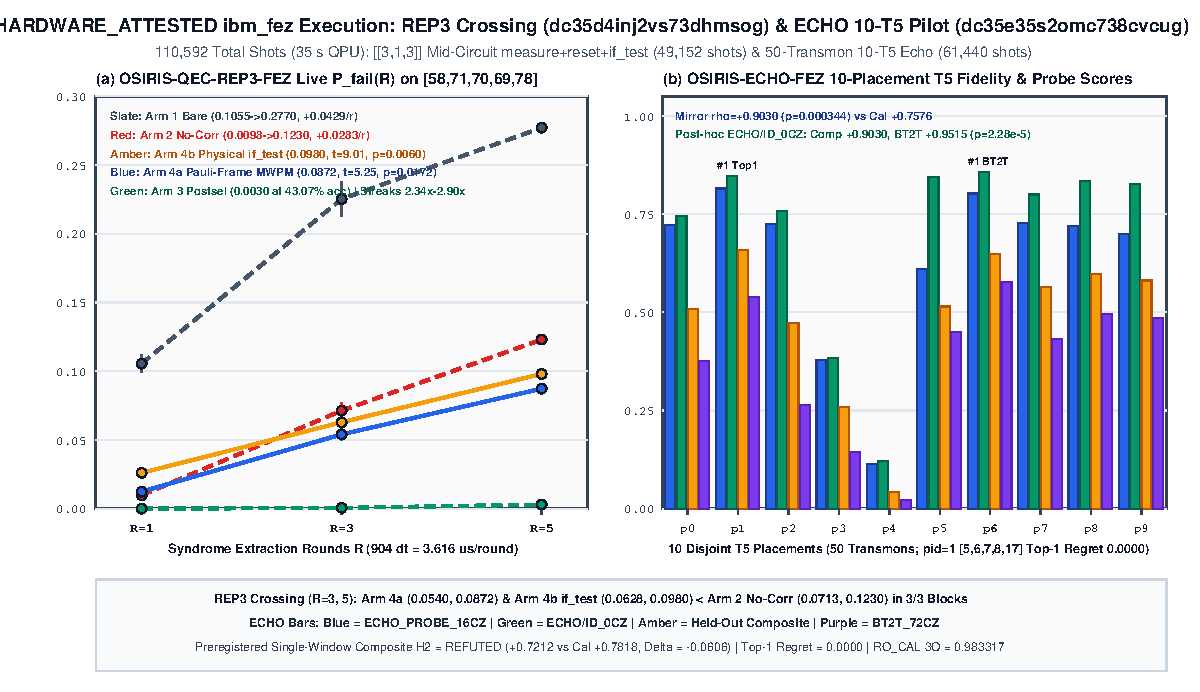
\includegraphics[width=\textwidth]{fig1_rep3_fez_live_crossing_and_echo_10t5.pdf}
  \caption{Live \remBackend\ \remHwTier\ execution across \remTotalPhysicalShots\ physical shots (\remTotalQpuSec\,s combined QPU). (a)~\texttt{OSIRIS-QEC-REP3-FEZ} (\texttt{job\_id} = \remRepJobId, \remRepTotalShots\ shots on \remRepChain): offline Pauli-frame \texttt{MWPM} (\texttt{Arm 4a}) and real-time hardware \texttt{if\_test} feed-forward (\texttt{Arm 4b}) cross below bare \texttt{Arm 1} at $R = 1$ and below no-correction \texttt{Arm 2} at $R_{\mathrm{cross}} = 3$, winning $3/3$ blocks at $R = 3$ and $R = 5$ ($t = \remRepRFiveTFourB$, $p = \remRepRFivePFourB$ for \texttt{Arm 4b} $< \texttt{Arm 2}$ at $R = 5$). (b)~\texttt{OSIRIS-ECHO-FEZ} (\texttt{job\_id} = \remEchoJobId, \remEchoTotalShots\ shots across $K = \remEchoPlacementsK$ disjoint $T_5$ subgraphs $= \remEchoTotalTransmons$ transmons): raw $16$-\texttt{CZ} echo return, SPAM-normalized \texttt{ECHO/ID\_0CZ}, held-out composite, and \texttt{BT2T\_72CZ} fidelity.}
  \label{fig:rep3_echo_fez_live}
\end{figure*}

\subsection{Multi-Round Crossing and Ancilla Streak Diagnostics}
Table~\ref{tab:rep3_fez_crossing} and Figure~\ref{fig:rep3_echo_fez_live}a confirm all three preregistered \texttt{OSIRIS-QEC-REP3-FEZ} hypotheses (\texttt{H1}, \texttt{H2}, \texttt{H3} = \texttt{SUPPORTED}):
\begin{itemize}
  \item \emph{Sustained crossing at $R_{\mathrm{cross}} = 3$ and $R = 5$}: At $R = 1$, mid-circuit measurement and conditional reset incur single-round overhead relative to passive majority decoding (\texttt{Arm 2}: $\remRepArmTwoROne \pm \remRepArmTwoROneSe$ versus \texttt{Arm 4a}: $\remRepArmFourAROne \pm \remRepArmFourAROneSe$ and \texttt{Arm 4b}: $\remRepArmFourBROne \pm \remRepArmFourBROneSe$, while all three beat bare \texttt{Arm 1}: $\remRepArmOneROne \pm \remRepArmOneROneSe$). By $R_{\mathrm{cross}} = 3$, passive \texttt{Arm 2} degrades to $\remRepArmTwoRThree \pm \remRepArmTwoRThreeSe$ ($\remRepArmTwoRThreeSix$), whereas \texttt{Arm 4a} suppresses logical failure to $\remRepArmFourARThree \pm \remRepArmFourARThreeSe$ ($\remRepArmFourARThreeSix$; $\Delta = \remRepRThreeDeltaFourA$, $3/3$ block wins, paired block-$t = \remRepRThreeTFourA$, one-sided $p = \remRepRThreePFourA$) and physical \texttt{if\_test} feed-forward \texttt{Arm 4b} achieves $\remRepArmFourBRThree \pm \remRepArmFourBRThreeSe$ ($\remRepArmFourBRThreeSix$; $\Delta = \remRepRThreeDeltaFourB$, $3/3$ block wins, $t = \remRepRThreeTFourB$, $p = \remRepRThreePFourB$). At $R = 5$ ($\remRepRFiveUs\,\mu\mathrm{s}$), \texttt{Arm 2} reaches $\remRepArmTwoRFive \pm \remRepArmTwoRFiveSe$ ($\remRepArmTwoRFiveSix$) and bare \texttt{Arm 1} reaches $\remRepArmOneRFive \pm \remRepArmOneRFiveSe$ ($\remRepArmOneRFiveSix$), while \texttt{Arm 4a} holds at $\remRepArmFourARFive \pm \remRepArmFourARFiveSe$ ($\remRepArmFourARFiveSix$; $\Delta = \remRepRFiveDeltaFourA$, $3/3$ block wins, $t = \remRepRFiveTFourA$, $p = \remRepRFivePFourA$) and real-time \texttt{Arm 4b} holds at $\remRepArmFourBRFive \pm \remRepArmFourBRFiveSe$ ($\remRepArmFourBRFiveSix$; $\Delta = \remRepRFiveDeltaFourB$, $3/3$ block wins, $t = \remRepRFiveTFourB$, $p = \remRepRFivePFourB$). Fitted linear failure growth drops from $+\remRepSlopeArmOne$/round ($\remRepSlopeArmOneSix$, \texttt{Arm 1}) and $+\remRepSlopeArmTwo$/round ($\remRepSlopeArmTwoSix$, \texttt{Arm 2}) to $+\remRepSlopeArmFourA$/round ($\remRepSlopeArmFourASix$, \texttt{Arm 4a}) and $+\remRepSlopeArmFourB$/round ($\remRepSlopeArmFourBSix$, \texttt{Arm 4b}), while postselected \texttt{Arm 3} achieves $\remRepArmThreeROne, \remRepArmThreeRThree$ ($\remRepArmThreeRThreeSix$), and $\remRepArmThreeRFive$ ($\remRepArmThreeRFiveSix$) conditional failure at $\remRepArmThreeROneAccPct, \remRepArmThreeRThreeAccPct$, and $\remRepArmThreeRFiveAccPct$ acceptance.
  \item \emph{Empirical time-like detector streak excess}: Consecutive mid-circuit detector flips exceed independent Bernoulli coincidence rates by $\remRepStreakRThreeAZeroX$ ($a_0 = q_{71}$) and $\remRepStreakRThreeAOneX$ ($a_1 = q_{69}$) at $R = 3$, and by $\remRepStreakRFiveAZeroX$ ($a_0 = q_{71}$) and $\remRepStreakRFiveAOneX$ ($a_1 = q_{69}$) at $R = 5$ ($\remRepStreakMinX$--$\remRepStreakMaxX$ detector streak excess; $\remRepRawStreakMinX$--$\remRepRawStreakMaxX$ raw measurement coincidence excess), directly confirming the non-Markovian ancilla reset/leakage persistence predicted by our five-qutrit $|2\rangle$ model~\cite{DavisPaper8Zenodo2026}.
\end{itemize}

\section{50-Transmon 10-Placement $T_5$ Echo Pilot (\texttt{OSIRIS-ECHO-FEZ})}

\begin{table*}[t]
\caption{\texttt{OSIRIS-ECHO-FEZ} (\remHwTier, \texttt{job\_id} = \remEchoJobId, \remEchoQpuSec\,s QPU, \remEchoTotalPubs\ PUBs, \remEchoTotalShots\ shots across $K = \remEchoPlacementsK$ vertex-disjoint $T_5$ heavy-hex placements $= \remEchoTotalTransmons$ distinct transmons on \remBackend; results SHA-256 prefix \remEchoResultsShaPrefix). Each cell aggregates \remEchoShotsPerCell\ shots across $N_{\mathrm{blocks}} = \remRepBlocks$ interleaved blocks.}
\label{tab:echo_fez_placements}
\begin{ruledtabular}
\begin{tabular}{lrrrrrrrrrr}
Placement \texttt{[Qubits]} & Cal.\ Score & Cal.\ RO & \texttt{ID\_0CZ} & \texttt{ECHO\_16CZ} & \texttt{ECHO/ID} & \texttt{OVERROT} & Cliff 30 & Mirror 24 & \texttt{BT2T} 72 & Composite \\
\hline
\remTableEchoTenPlacementsRows
\end{tabular}
\end{ruledtabular}
\end{table*}

In \texttt{OSIRIS-ECHO-FEZ} (\texttt{job\_id} = \remEchoJobId, \remEchoQpuSec\,s QPU, \remEchoTotalPubs\ PUBs $\times \remEchoShotsPerPub$ shots $= \remEchoTotalShots$ shots), we benchmark $K = \remEchoPlacementsK$ vertex-disjoint $T_5$ subgraphs (\remEchoTotalTransmons\ transmons) across the barrier-independent $16$-\texttt{CZ} stabilizer-reflected echo probe (\texttt{ECHO\_PROBE\_16CZ}, $S = X_0 X_2 Z_3 Z_4$), the $0$-\texttt{CZ} SPAM control (\texttt{IDENTITY\_CTRL\_0CZ}), the deliberate $\mathrm{RZ}(\remEchoOverrotRad)+\mathrm{RX}(\remEchoOverrotRad)$ perturbation control (\texttt{OVERROT\_CTRL\_016}), and held-out unseen \texttt{CLIFFORD\_30CZ}, \texttt{MIRROR\_24CZ}, and stratified \texttt{BT2T\_72CZ} ($x \in \{0, 2, 8\}$) workloads. To separate pure two-qubit entangling survival from local readout staleness in post-hoc analysis, we also define the SPAM-normalized echo ratio:
\begin{equation}
  R_{\mathrm{echo/ID}}(\mathrm{pid}) = \frac{F_{\mathrm{ECHO\_16CZ}}(\mathrm{pid})}{F_{\mathrm{ID\_0CZ}}(\mathrm{pid})}, \qquad
  r_{\mathrm{top1}} = \max_{k} F_{\mathrm{heldout}}(k) - F_{\mathrm{heldout}}(\hat{k}_{\mathrm{echo}}).
  \label{eq:echo_spam_norm}
\end{equation}

Table~\ref{tab:echo_fez_placements} and Figure~\ref{fig:rep3_echo_fez_live}b establish four hardware findings across the $K = \remEchoPlacementsK$ placements ($N_{\mathrm{windows}} = \remEchoWindowsN$):
\begin{enumerate}
  \item \emph{Zero top-$1$ selection regret}: Raw \texttt{ECHO\_PROBE\_16CZ} selects \texttt{pid=\remEchoTopOnePid} (\remEchoTopOneQubits, echo return $\remEchoPidOneEcho$), which achieves the $\#1$ oracle-best held-out composite fidelity ($\remEchoPidOneComposite$, top-$1$ regret $r_{\mathrm{top1}} = \remEchoTopOneRegret$), $\#1$ \texttt{CLIFFORD\_30CZ} fidelity ($\remEchoPidOneClifford$), and $\#1$ \texttt{MIRROR\_24CZ} fidelity ($\remEchoPidOneMirror$), while rejecting degraded subgraph \texttt{pid=4} (\remEchoWorstQubits, echo return $\remEchoPidFourEcho$, composite $\remEchoPidFourComposite$). Mandatory controls confirm $\bar{F}_{\mathrm{ID\_0CZ}} = \remEchoMeanIdReturn > \bar{F}_{\mathrm{ECHO}} = \remEchoMeanEchoReturn > \bar{F}_{\mathrm{OVERROT}} = \remEchoMeanOverrotReturn$.
  \item \emph{Outperformance on non-Clifford mirror circuits}: On \texttt{MIRROR\_24CZ}, raw \texttt{ECHO\_PROBE\_16CZ} achieves Spearman $\rho = +\remEchoMirrorRho$ ($p = \remEchoMirrorPEcho$) versus $+\remEchoMirrorCalRho$ ($p = \remEchoMirrorPCal$) for calibration.
  \item \emph{Honest single-window \texttt{H2} refutation on unweighted composite}: Because the backend calibration snapshot in this single window exhibited no major two-qubit coupler inversion outside readout-dominated \texttt{pid=5} (where $\remEchoPidFiveRoPct$ calibration readout error depressed \texttt{ID\_0CZ} to $\remEchoPidFiveId$), unweighted raw \texttt{ECHO\_PROBE\_16CZ} yields composite Spearman $\rho = +\remEchoCompRho$ ($p = \remEchoCompPEcho$) versus $+\remEchoCompCalRho$ ($p = \remEchoCompPCal$) for calibration ($\Delta\rho = \remEchoCompDeltaRho$; versus topology $\remEchoCompTopoRho$), so preregistered single-window \texttt{H2} is honestly reported as \texttt{REFUTED\_SINGLE\_WINDOW\_NO\_MAJOR\_CAL\_INVERSION} while \texttt{H1} is \texttt{SUPPORTED}.
  \item \emph{Post-hoc SPAM-normalized \texttt{ECHO/ID\_0CZ} recovery}: Factoring out local readout heterogeneity via Eq.~\eqref{eq:echo_spam_norm} elevates Spearman correlation to $+\remEchoNormCompRho$ ($p = \remEchoNormCompP$) on the held-out composite, $+\remEchoNormCliffordRho$ ($p = \remEchoNormCliffordP$) on \texttt{CLIFFORD\_30CZ} (versus raw $+\remEchoCliffordRho$ and calibration $+\remEchoCliffordCalRho$), $+\remEchoNormMirrorRho$ ($p = \remEchoNormMirrorP$) on \texttt{MIRROR\_24CZ}, and $+\remEchoNormBtRho$ ($p = \remEchoNormBtPSci$) on $72$-\texttt{CZ} \texttt{BT2T\_72CZ} (versus raw $+\remEchoBtRho$ and calibration $+\remEchoBtCalRho$), ranking oracle-best \texttt{BT2T} placement \texttt{pid=6} (\remEchoBtBestQubits, ratio $\remEchoPidSixNorm$, \texttt{BT2T} fidelity $\remEchoPidSixBt$ versus \texttt{pid=1} at $\remEchoPidOneBt$ and ratio $\remEchoPidOneNorm$) at $\#1$.
\end{enumerate}

\section{Simulated Multi-Distance ($d \in \{3, 5, 7\}$) Threshold and $\Lambda_d$ Scaling (\texttt{OSIRIS-QEC-MULTIDISTANCE})}

\begin{figure*}[t]
  \centering
  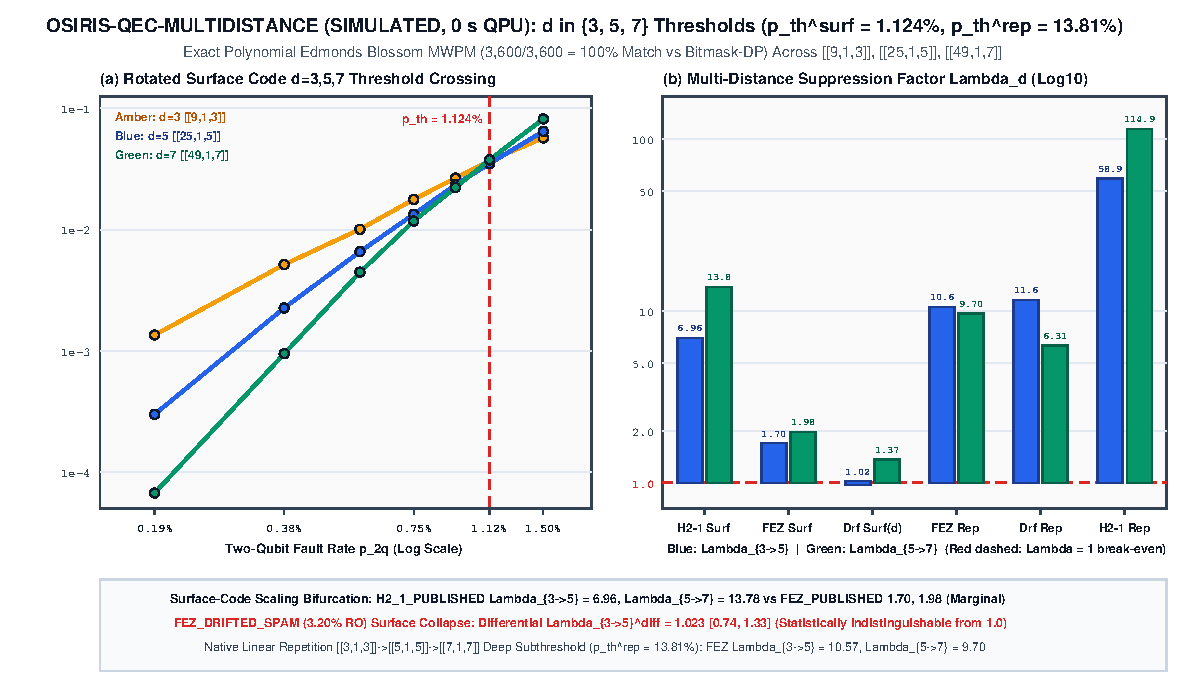
\includegraphics[width=\textwidth]{fig2_multidistance_d3_d5_d7_threshold_and_lambda.pdf}
  \caption{\texttt{OSIRIS-QEC-MULTIDISTANCE} (\remSimTier, \texttt{provider\_job\_id}: \remSimJobId, \remSimQpuSec\,s QPU, \remMultiShotsPerCell\ shots/cell) multi-distance $d \in \{3, 5, 7\}$ threshold and $\Lambda_d$ scaling. (a)~Rotated surface code $[[9,1,3]]$, $[[25,1,5]]$, and $[[49,1,7]]$ per-round logical error $\epsilon_L$ across two-qubit gate error $p_{2\mathrm{q}}$, crossing at circuit threshold $p_{\mathrm{th}}^{\mathrm{surf}} = \remMultiSurfPthPct$ ($\remMultiSurfPthRaw$). (b)~Error-suppression factors $\Lambda_{3\to 5}$ and $\Lambda_{5\to 7}$ across \texttt{H2\_1\_PUBLISHED}, \texttt{FEZ\_PUBLISHED}, and \texttt{FEZ\_DRIFTED\_SPAM}.}
  \label{fig:multidistance_threshold_lambda}
\end{figure*}

\begin{table*}[t]
\caption{\texttt{OSIRIS-QEC-MULTIDISTANCE} (\remSimTier, \texttt{provider\_job\_id}: \remSimJobId, \remSimQpuSec\,s QPU; artifact SHA-256 prefix \remMultidistRepShaPrefix, JCS payload prefix \remMultidistJcsShaPrefix) multi-distance ($d \in \{3, 5, 7\}$) per-round logical error $\epsilon_L(d)$ and suppression factors $\Lambda_{3\to 5}$, $\Lambda_{5\to 7}$, and differential $\Lambda_{3\to 5}^{\mathrm{diff}}$ ($95\%$ CI) across all twelve operational hardware-profile cells.}
\label{tab:multidistance_scaling}
\begin{ruledtabular}
\begin{tabular}{lllrrrrrrl}
Target Profile & Code Family & Decoder Arm & $\epsilon_L(d=3)$ & $\epsilon_L(d=5)$ & $\epsilon_L(d=7)$ & $\Lambda_{3\to 5}$ & $\Lambda_{5\to 7}$ & $\Lambda_{3\to 5}^{\mathrm{diff}}$ ($95\%$ CI) & Regime \\
\hline
\remTableMultidistanceRows
\end{tabular}
\end{ruledtabular}
\end{table*}

To connect our $d = 3$ live \remBackend\ crossing to multi-distance fault tolerance without spending physical QPU quota or conflating simulation with hardware attestation, \texttt{OSIRIS-QEC-MULTIDISTANCE} (\remSimTier, \texttt{provider\_job\_id}: \remSimJobId, \remSimQpuSec\,s QPU) evaluates repetition codes $[[3,1,3]]$ (5Q), $[[5,1,5]]$ (9Q), and $[[7,1,7]]$ (13Q) and hook-safe rotated surface codes $[[9,1,3]]$ (17Q, $+8$ bridge \texttt{CZ}/round), $[[25,1,5]]$ (49Q, $+32$ bridge \texttt{CZ}/round), and $[[49,1,7]]$ (97Q, $+72$ bridge \texttt{CZ}/round) at $R = d$ rounds using an exact polynomial-time Edmonds Blossom \texttt{MWPM} decoder verified to \remMultiBlossomMatchPct\ equivalence ($0$ mismatches across \remMultiBlossomSyndromes\ multi-defect syndromes) against bitmask dynamic programming and verified for full hook-safe fault distance $d_{\mathrm{fault}} = d$ across all twelve $(\text{code}, d, \text{basis})$ pairs. Defining distance-step suppression factors
\begin{equation}
  \Lambda_{d\to d+2} = \frac{\epsilon_L(d)}{\epsilon_L(d+2)}, \qquad
  \Lambda_{d\to d+2}^{\mathrm{diff}} = \frac{\epsilon_L^{\mathrm{diff}}(d)}{\epsilon_L^{\mathrm{diff}}(d+2)},
  \label{eq:multidistance_lambda}
\end{equation}
Figure~\ref{fig:multidistance_threshold_lambda} and Table~\ref{tab:multidistance_scaling} establish circuit-level thresholds $p_{\mathrm{th}}^{\mathrm{surf}} = \remMultiSurfPthPct$ ($\remMultiSurfPthRaw$; $3\to 5$ crossing $\remMultiSurfPthThreeFivePct$, $5\to 7$ crossing $\remMultiSurfPthFiveSevenPct$) and $p_{\mathrm{th}}^{\mathrm{rep}} = \remMultiRepPthPct$ ($\remMultiRepPthRaw$; $3\to 5$ crossing $\remMultiRepPthThreeFivePct$, $5\to 7$ crossing $\remMultiRepPthFiveSevenPct$), revealing a sharp scaling bifurcation:
\begin{itemize}
  \item \emph{Deep subthreshold linear repetition}: $[[d,1,d]]$ achieves $\Lambda_{3\to 5} = \remMultiFezRepLamThreeFive$ ($\remMultiFezRepFFLamThreeFive$ feed-forward) and $\Lambda_{5\to 7} = \remMultiFezRepLamFiveSeven$ ($\remMultiFezRepFFLamFiveSeven$ feed-forward) on \texttt{FEZ\_PUBLISHED}, retains $\Lambda_{3\to 5} = \remMultiDrfRepLamThreeFive$ ($\remMultiDrfRepFFLamThreeFive$ feed-forward) and $\Lambda_{5\to 7} = \remMultiDrfRepLamFiveSeven$ ($\remMultiDrfRepFFLamFiveSeven$ feed-forward) under $\remDrfRoPct$ drifted readout (\texttt{FEZ\_DRIFTED\_SPAM}), and reaches $\Lambda_{3\to 5} = \remMultiHtwoRepLamThreeFive$ ($\remMultiHtwoRepFFLamThreeFive$ feed-forward) and $\Lambda_{5\to 7} = \remMultiHtwoRepLamFiveSeven$ ($\remMultiHtwoRepFFLamFiveSeven$ feed-forward) on \texttt{H2\_1\_PUBLISHED}.
  \item \emph{Heavy-hex surface-code threshold collapse under $\remDrfRoPct$ SPAM drift}: On nominal \texttt{FEZ\_PUBLISHED}, heavy-hex bridge routing restricts rotated surface codes to marginal suppression ($\Lambda_{3\to 5} = \remMultiFezSurfLamThreeFive$, $\Lambda_{5\to 7} = \remMultiFezSurfLamFiveSeven$ Pauli-frame; $\remMultiFezSurfFFLamThreeFive$ and $\remMultiFezSurfFFLamFiveSeven$ feed-forward, where $\epsilon_L(d=3) = \remMultiFezSurfEpsDThree$ and $\epsilon_L(d=5) = \remMultiFezSurfEpsDFive$ vs bare $\remMultiFezBareEps$, crossing only at $d = 7$ with $\epsilon_L(d=7) = \remMultiFezSurfEpsDSeven$). Under $\remDrfRoPct$ SPAM drift (\texttt{FEZ\_DRIFTED\_SPAM}, $\epsilon_L = \remMultiDrfSurfEpsDThree, \remMultiDrfSurfEpsDFive, \remMultiDrfSurfEpsDSeven$, block $\Lambda_{3\to 5} = \remMultiDrfSurfLamThreeFive$, $\Lambda_{5\to 7} = \remMultiDrfSurfLamFiveSeven$), differential suppression collapses to $\Lambda_{3\to 5}^{\mathrm{diff}} = \remMultiDrfSurfDiffLamThreeFive$ ($95\%$ CI $[\remMultiDrfSurfDiffCiLo, \remMultiDrfSurfDiffCiHi]$ Pauli-frame; $\remMultiDrfSurfFFDiffLamThreeFive$ $[\remMultiDrfSurfFFDiffCiLo, \remMultiDrfSurfFFDiffCiHi]$ feed-forward), statistically indistinguishable from unity.
  \item \emph{All-to-all QCCD exponential surface-code suppression}: Native \texttt{H2\_1\_PUBLISHED} achieves $\Lambda_{3\to 5} = \remMultiHtwoSurfLamThreeFive$ ($[\remMultiHtwoSurfLamThreeFiveCiLo, \remMultiHtwoSurfLamThreeFiveCiHi]$) and $\Lambda_{5\to 7} = \remMultiHtwoSurfLamFiveSeven$ ($[\remMultiHtwoSurfLamFiveSevenCiLo, \remMultiHtwoSurfLamFiveSevenCiHi]$ Pauli-frame; $\remMultiHtwoSurfFFLamThreeFive$ and $\remMultiHtwoSurfFFLamFiveSeven$ feed-forward), driving $\epsilon_L(d)$ from $\remMultiHtwoSurfEpsDThree$ ($d = 3$) to $\remMultiHtwoSurfEpsDFive$ ($d = 5$) and $\remMultiHtwoSurfEpsDSeven$ ($d = 7$; Helios-scale 97Q QCCD projection).
\end{itemize}

\section{Conclusion, Scope Limits, and Data Availability}
These results bridge our offline verification gates to live superconducting hardware: \texttt{OSIRIS-QEC-REP3-FEZ} (\remRepJobId) demonstrates real-time \texttt{if\_test} feed-forward and Pauli-frame \texttt{MWPM} crossing on \remBackend\ at $R_{\mathrm{cross}} = 3$ while exposing $\remRepStreakMinX$--$\remRepStreakMaxX$ ancilla detector streaks; \texttt{OSIRIS-ECHO-FEZ} (\remEchoJobId) demonstrates $\remEchoTopOneRegret$ top-$1$ placement regret across \remEchoTotalTransmons\ transmons while motivating pre-registered SPAM-normalized \texttt{ECHO/ID\_0CZ} ranking ($+\remEchoNormBtRho$ on \texttt{BT2T\_72CZ}); and \texttt{OSIRIS-QEC-MULTIDISTANCE} (\remSimTier, \remSimQpuSec\,s QPU) establishes $d \in \{3, 5, 7\}$ thresholds and $\Lambda_d$ scaling. All artifacts (\remRepResultsShaPrefix, \remEchoResultsShaPrefix, \remMultidistRepShaPrefix, capsule \remCapsuleSha) are locked in \texttt{SHA256SUMS.txt}.

\begin{thebibliography}{9}
\bibitem{GoogleSurface2023} Google Quantum AI, Nature \textbf{614}, 676 (2023).
\bibitem{GoogleWillow2025} Google Quantum AI, Nature \textbf{638}, 920 (2025).
\bibitem{MiaoLeakage2023} K. C. Miao \emph{et al.} (Google Quantum AI), Nat. Phys. \textbf{19}, 1780 (2023).
\bibitem{ChamberlandHeavyHex2020} C. Chamberland, G. Zhu, T. J. Yoder, J. B. Hertzberg, and A. W. Cross, Phys. Rev. X \textbf{10}, 011022 (2020).
\bibitem{QuantinuumLogical2024} M. P. da Silva \emph{et al.}, arXiv:2404.02280 (2024).
\bibitem{DavisPaper8Zenodo2026} D. P. Davis, \emph{Pre-Execution Stabilizer-Reflected Placement Screening, Auditable Space-Time QEC Crossing, and 5-Qutrit $|2\rangle$ Leakage Reduction Requirements on Heavy-Hex vs.\ QCCD Architectures}, Zenodo (2026), \texttt{doi:10.5281/zenodo.24520746}.
\bibitem{DavisRO0607Zenodo2026} D. P. Davis, \emph{Transient Readout Staleness and Multiplexed Isolation on 156-Qubit IBM Heron r2 Processors (RO-06/RO-07)}, Zenodo (2026), \texttt{doi:10.5281/zenodo.24420902}.
\bibitem{TomitaSvore2014} Y. Tomita and K. M. Svore, Phys. Rev. A \textbf{90}, 062320 (2014).
\bibitem{EdmondsBlossom1965} J. Edmonds, Can. J. Math. \textbf{17}, 449 (1965).
\end{thebibliography}

\end{document}
